\section{Evaluation}
\subsection{Techniques used for the evaluation}
All calculations in this section are done with scripts written in 
the \textit{python} programming language~\cite{python}, relaying in several 
packages:
\begin{itemize}
    \item
        \textit{matplotlib}~\cite{Hunter2007} for plotting,
    \item
        \textit{scipy}~\cite{scipy} for fitting, and 
    \item
        \textit{uncertainties}~\cite{uc} for error propagation.
\end{itemize}
The latter applies gaussian error propagation for correlated and uncorrelated variables. 
We will thus not explicitly write down the formulas for the error propagation 
for each quantity calculated but instead state the numerical result, only. 
We will, however make a quick remark on the use of covariance matrices in 
error propagation: Contrary to measured data, which in our case is usually 
expected to be uncorrelated, all fitted data yields variables that in general correlate. 
The propagation is then done as follows:
Let's assume we have random
variables $x_0,...,x_N$ which are correlated through the $N\times N$ Matrix $cov(x_i,x_j)$.
For a scalar function $f(x_0,...,x_N) \rightarrow \mathbb{R}$, the variance is estimated (linearly) by:
\begin{equation}
Var[f] = \sigma^2 = \sum_{i,j} \frac{\partial f}{\partial x_i} \frac{\partial f}{\partial x_j} cov(x_i,x_j) \,.
\end{equation} 
If instead, $\mathbf{f}$ is a vector field in $m$ dimensions, namely 
$\mathbf{f}(x_0,...,x_N) \rightarrow \mathbb{R}^m$, then the components of $\mathbf{f}$ 
are further correlated. We can write down the relation between the covariance matrices $V$ and $U$ of 
$\mathbf{x}$ and $\mathbf{f}$, respectively, in matrix relations:
\begin{equation}
    U = A V A^T
\end{equation}
where $A$ is the matrix defined by 
\begin{equation}
    A_{ij} = \left[ \frac{\partial f_i}{\partial x_j}\right]_{\mathbf{x} = \mathbf{\mu}}
\end{equation}
with expectation value $E[\mathbf{x}] = \mathbf{\mu}$.~\cite{cowan1998statistical}
In order to facilitate notation, the covariance matrices will in general be notated without 
specifying the units. If not specified explicitly, the units will correspond to those of the
variables: If $x_i, x_j$ have the units $[x_i], [x_j]$, respectively, 
then the entry of the covariance matrix has the unit $[x_i] \cdot [x_j]$. 



\subsection{Band Gap}
The raw data is plotted in figure \ref{fig:band_gap_raw_Ge} for 
germanium and \ref{fig:band_gap_raw_Si} for silicon. 
We set the $U-I$-converter to $15.03 \pm 0.03\,$mA for Ge 
and $0.75 \pm 0.01\,$mA for Si. The aperture was opened to 
$-10.0$--$+10.0\,$mm for both samples. Further settings 
not relevant for the evaluation, such as the settings of the gains, 
can be looked up in the 
handwritten records of the experiment in the appendix, 
\ref{sec:records_band_gap}. 
\begin{figure}
    \centering
    \begin{subfigure}[b]{\pltw}
        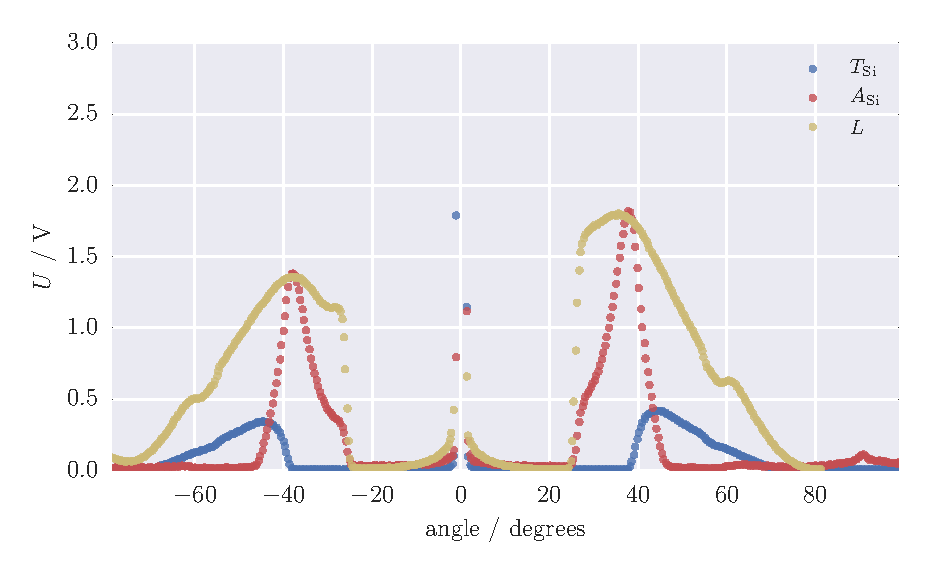
\includegraphics[width=1.0\linewidth]{figures/band_gap_raw_Si}
        \caption{}
        \label{fig:band_gap_raw_Si}
    \end{subfigure}
    \begin{subfigure}[b]{\pltw}
        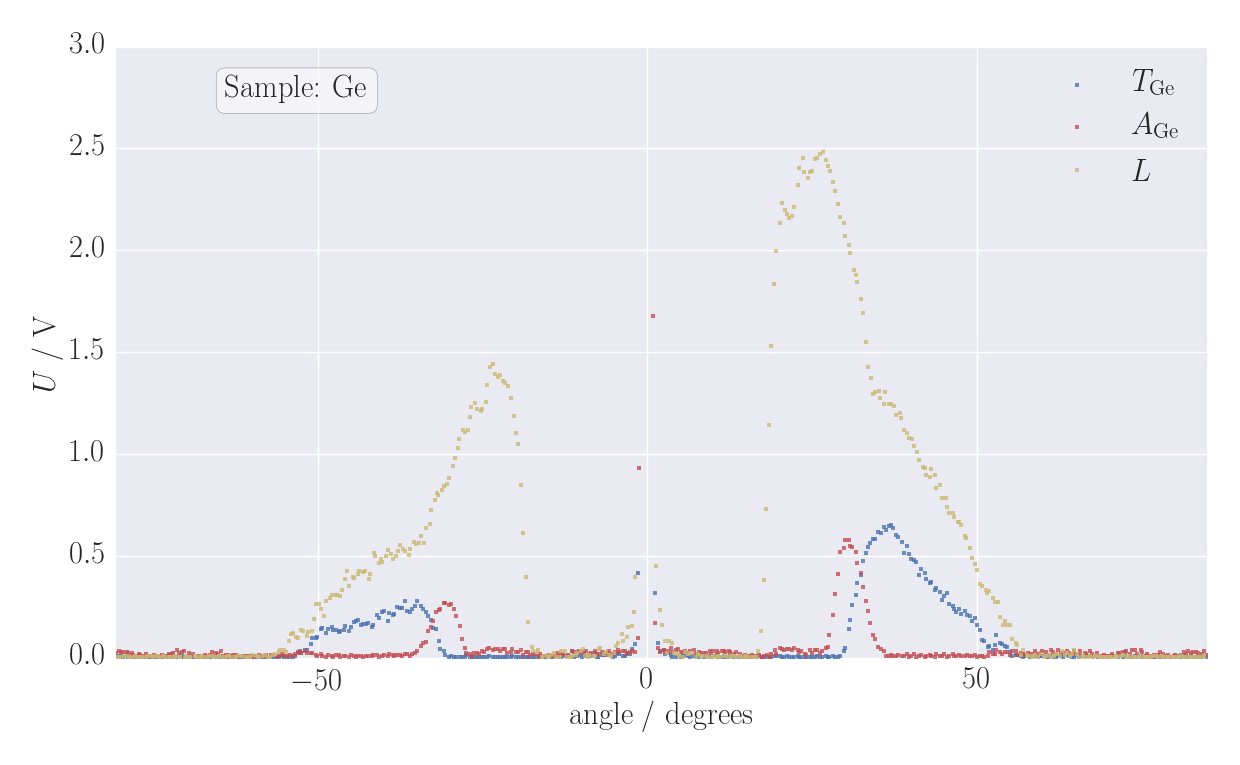
\includegraphics[width=1.0\linewidth]{figures/band_gap_raw_Ge}
        \caption{}
        \label{fig:band_gap_raw_Ge}
    \end{subfigure}
    \caption{
        The signals measured with Si (\ref{fig:band_gap_raw_Si}) 
        and Ge (\ref{fig:band_gap_raw_Ge}) as samples with corresponding 
        grating and filter. $T$ and $A$ indicate 
        the transmission and absorption, measured by the currents through 
        the pyrodetector and the semiconductor, respectively. 
        $L$ is the intensity of the lamp with installed filter, measured 
        without the semiconductor. The asymmetry might be due to 
        irregularities on the grating or within the beam path. 
        }
    \label{fig:band_gap}
\end{figure}
The evaluation for both samples is done 
absolutely analogously. We thus explain the steps for the example 
of Si plotting all necessary steps, while the plots for 
Ge are added to the appendix, \ref{sec:appendix_band_gap_plots}.
To go on, we perform an approximation on the errors. For the 
left side of the spectrum with the Si sample, we 
did five repetitive measurements. To approximate the fluctuations 
and errors resulting from uncertainties in the angle, 
we calculate the standard deviation of the values measured 
in each angle $\phi_i$. However, to do so we had to 
interpolate the data to obtain a new set of data on 
on one fixed grid, because the angles measured in each set did not agree. 
From each data set, e.~g. angles $\phi$ as well as measured transmission $T$ 
and absorption $A$ with the Si sample installed, we created a traverse function 
interpolating $T$ and $A$ on a predefined grid. 
Calculating $T$ at angle $\phi$ was done in the following manner:
Let $(\phi_1, T_1)$ and 
$(\phi_2, T_2)$ be the pairs of data point of one set with $\phi_1$ and $\phi_2$ the 
next angles on the left and right of $\phi$, respectively. 
Then, 
\begin{equation}
    T = \frac{1}{(\phi_2 - \phi_1)} 
        \left(T_1\left(\phi - \phi_1\right) + T_2\left(\phi_2 - \phi\right)\right)
\end{equation}
With this method we obtain arrays off only marginally reduced size but with 
equidistant steps. The information lost in this process is negligible since we 
don't observe high fluctuations in the original data. Furthermore, the following 
analysis does not crucially depend on possible fluctuations, either. 
The results are shown in figure~\ref{fig:band_gap_error}. One observes that the 
errors appear mostly in the regions of steeper descent or ascent -- clearly, 
they are due to the uncertainties in angles. 
\begin{figure}[htpb]
    \centering
    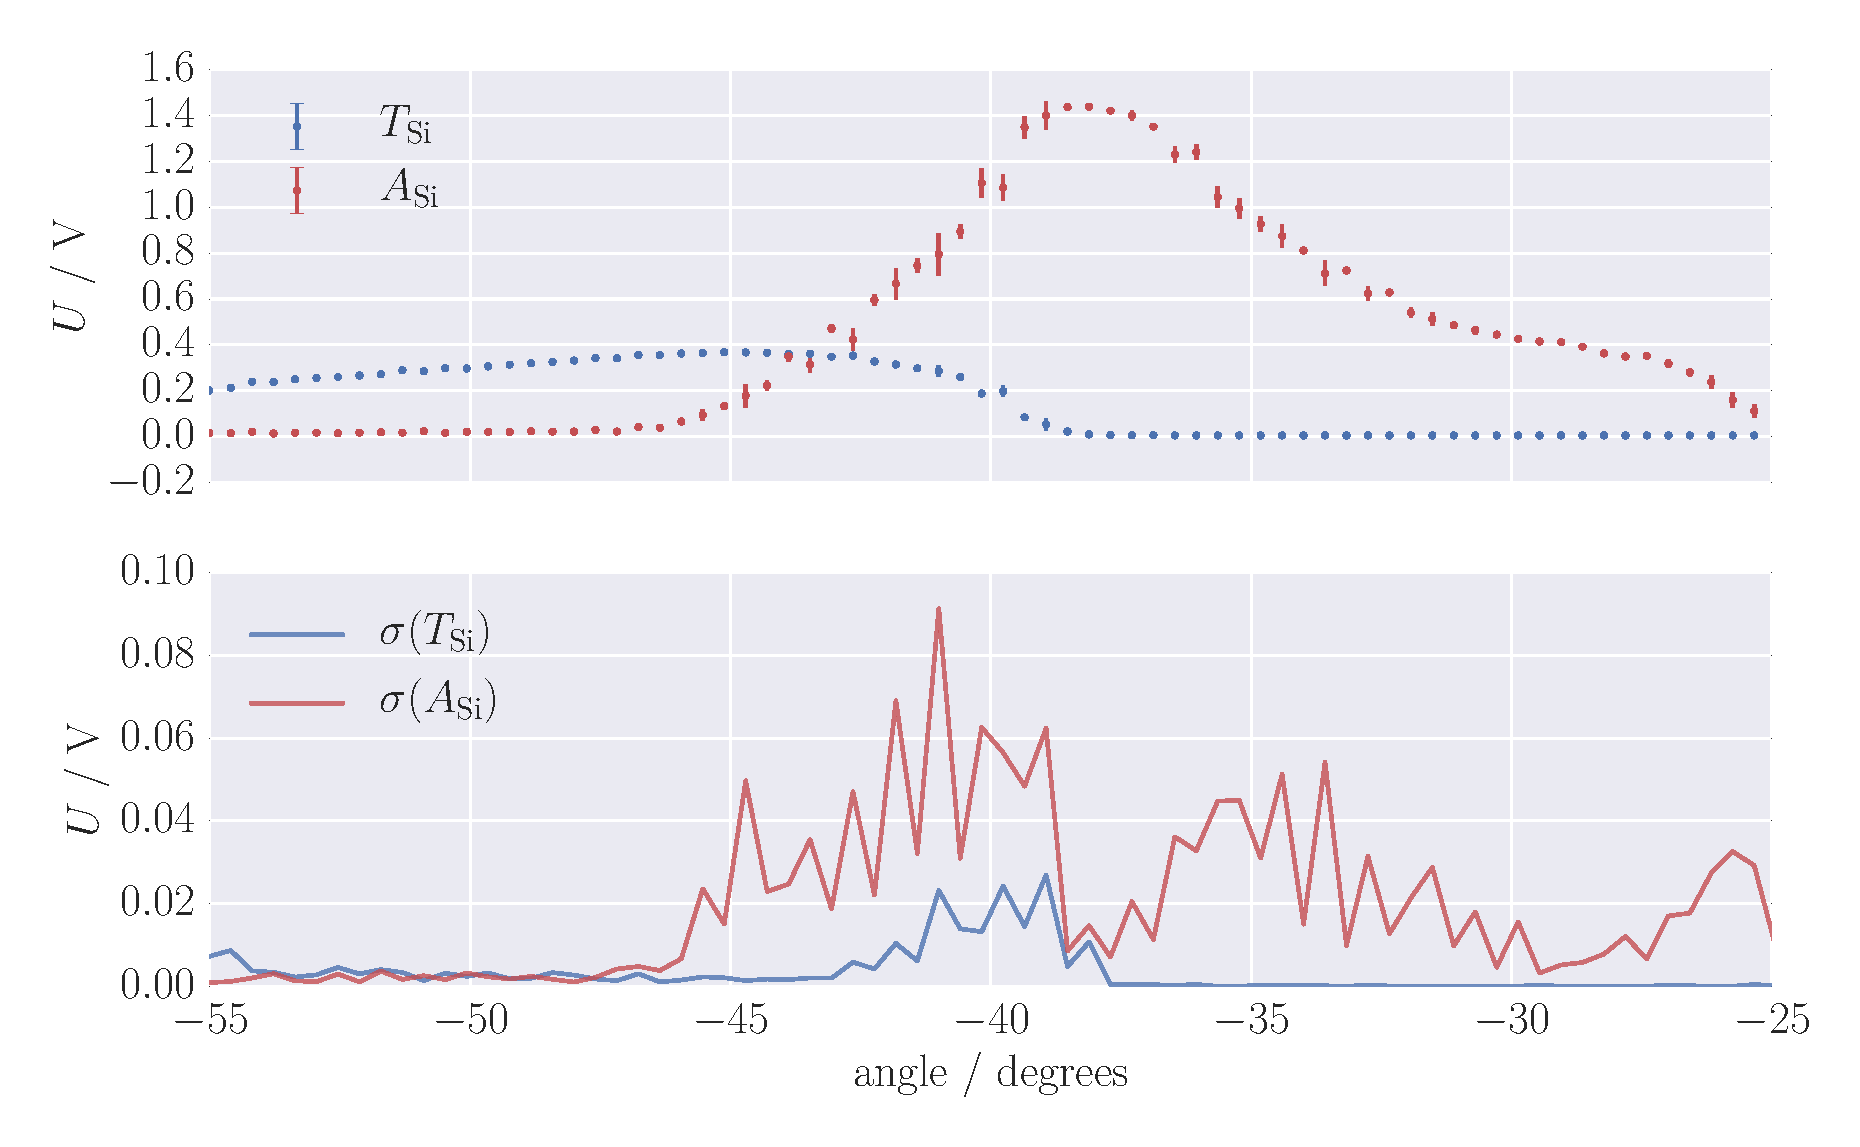
\includegraphics[width=1.0\linewidth]{figures/band_gap_error}
    \caption{
        Calculation of errors for the Si sample. The upper plot shows a single 
        measurement with the error bars obtained form the analysis of five successive 
        measurements of the same region. The lower one shows the amplitude of the errors. 
        It is clear that these errors stem from the errors in measuring the angle, 
        as they are much bigger in regions with larger slope. 
        Accordingly, the errors of the semiconductor signal (absorption)  appear 
        to be larger since it is subject to steeper ascending. 
        }
    \label{fig:band_gap_error}
\end{figure}
To obtain the corrected values of transmission and absorption, 
we apply the formulas \eqref{eq:t_real} and \eqref{eq:a_real}.
Again, the data had to be interpolated onto a predefined grid.
Seeking the intersect of the straight lines interpolated at the transition from 
absorption to transmission is done on a smaller scale. The
signals are normalized, setting $T = 1$ and $A = 1$ for the according maxima, 
when the antagonist is close to zero. The fit is then done choosing the 
points which are used manually. The results together with the points chosen for fitting 
are displayed in figure~\ref{fig:band_gap_result_Si_left}. 
\begin{figure}
    \centering
    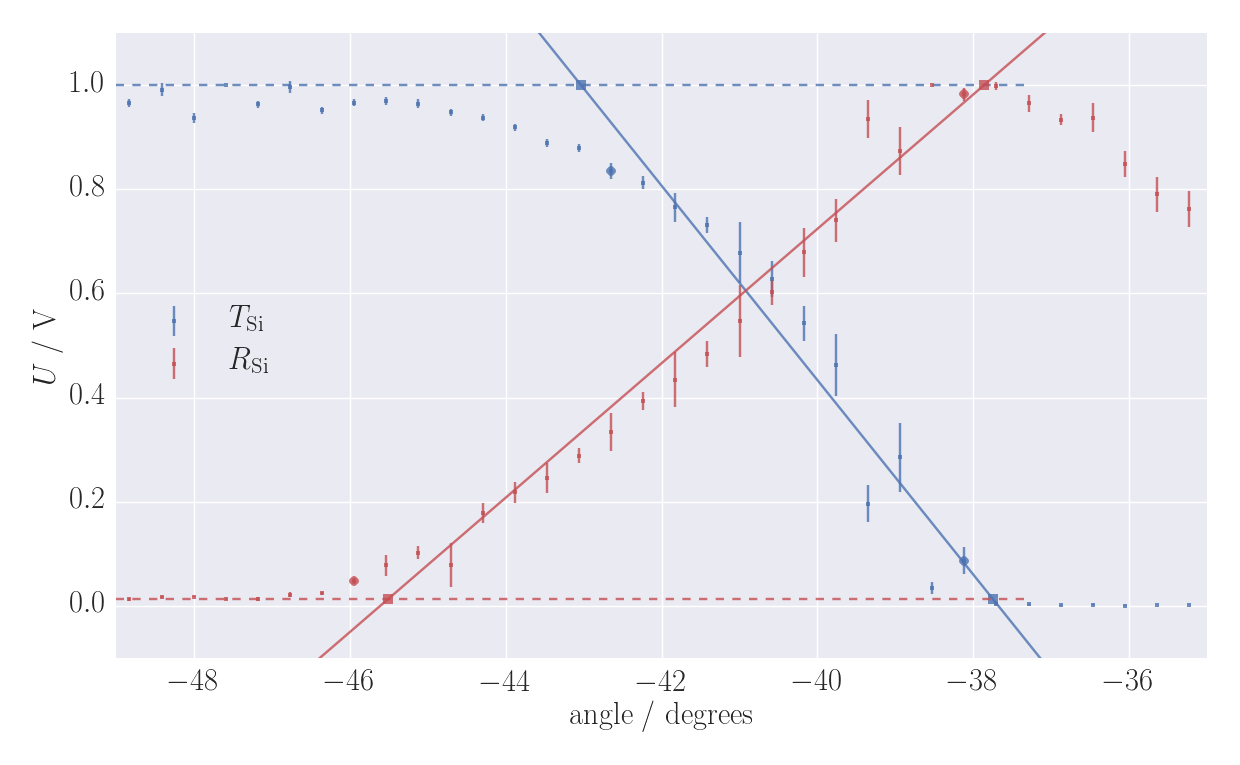
\includegraphics[width=1.0\linewidth]{figures/band_gap_result_error}
    \caption{
        Result of the procedure fitting straight lines through the points 
        at the transition from transmitting to absorbing characteristic for Si. 
        The larger round dots indicate the upper and lower limit 
        chosen for the interpolation. The dashed line corresponds to 
        the maximum of transmission and minimum of absorption, the 
        squares to the respective intersects with the straight lines.
        In order to maintain the clarity left
        the values for the angles at the intersects are given in the text. 
        The nominal value for the band gap energy is given by the intersect 
        of the two lines.
        The error bars indicate the propagated errors from the approximation. 
        Taking the mean values of the limits as uncertainties on the 
        value of the intersect, it is clear that including the propagated errors 
        does not change the final error significantly. 
        }
    \label{fig:band_gap_result_Si_left}
\end{figure}
The band gap energy is thus reached for an angle of $\phi_g = -41.0^\circ$, 
which applying equation~\eqref{eq:E_g} yields:
\begin{equation}
    E_g = \frac{h c}{2d |\sin(\phi)| \cos(\psi)} = 1.14\, \mathrm{eV}
\end{equation}
The error is obtained by taking the average of the tow boundaries on each side, 
which lie at 
\begin{align}
    \left.
    \begin{aligned}
        \phi_\mathrm{lower, 1} &= -37.8^\circ \\
        \phi_\mathrm{lower, 2} &= -38.0^\circ
    \end{aligned}
    \right\} \quad &\Rightarrow \quad
    \overline{\phi_\mathrm{lower}} = -37.9^\circ \\
    \left.
    \begin{aligned}
    \phi_\mathrm{upper, 1} &= -43.1^\circ \\
    \phi_\mathrm{upper, 2} &= -45.4^\circ
    \end{aligned}
    \right\} \quad &\Rightarrow \quad
    \overline{\phi_\mathrm{upper}} = -44.3^\circ \\
\end{align}
The resulting upper and lower boundaries are then given by
\begin{align}
    E_\mathrm{lower} = 1.22 \, \mathrm{eV} \\
    E_\mathrm{upper} = 1.07 \, \mathrm{eV}
\end{align}
(the index refers to the lower and upper angle, which leads to the 
    paradox nomenclature of $E_\mathrm{lower} > E_\mathrm{upper}$). 
The final result on the band gap energy of silicon are then
\begin{equation}
    E_g = (1.14 \pm 0.08) \, \mathrm{eV} \, ,
\end{equation}
where the absolute error is the maximal difference between the nominal value 
and the boundaries. 
This procedure is repeated analogously for the other side of the Si spectrum, 
and the germanium on both sides. 
The corresponding plots are shown in the appendix, 
figure~\ref{fig:band_gap_result_Si_right} for Si, followed by those for the 
germanium (\ref{fig:band_gap_result_Ge_left}, \ref{fig:band_gap_result_Ge_right}). 
The error bars are missing, since we only did the assessment for the Si in order to 
show the order of magnitude of the error, assuming it does not change dramatically for the 
germanium probe. 
The results are displayed in table \ref{tab:band_gap_results}, leaving out 
the single steps being connected to trivial numerical calculations. 
Taking the weighted average for the two measurements, we obtain:
\begin{align}
    \bar{E} &= \frac{ \sum_{i=1}^n \left( E_i \sigma_i^{-2} \right)}{\sum_{i=1}^n \sigma_i^{-2}} \qquad \text{(weighted mean)} \\
    \overline{E_{g, \mathrm{Si}}} &= (1.14 \pm 0.05) \,\mathrm{eV} \\
    \overline{E_{g, \mathrm{Ge}}} &= (0.69 \pm 0.03) \,\mathrm{eV}
\end{align}
The relative errors are with approximately 4 \% surprisingly small -- when learning about 
the applied method, we expected errors of much higher magnitude. 
Comparison to literature values~\cite{kittel1976introduction}, namely
\begin{align}
    E_\mathrm{Si, Lit} &= 1.11 \, \mathrm{ev} \\
    E_\mathrm{Ge, Lit} &= 0.66 \, \mathrm{ev} \, ,
\end{align}
shows that the measured values cover the accepted values just within the given uncertainty. 
Approximating the errors by the method applied thus did yield a realistic range. 
Systematic errors from offsets measuring the angle should be accounted for taking the 
average of the values obtained on both sides. There is no certain knowledge about 
further errors introduced by the electronics and other parts of the setup. 

\renewcommand{\arraystretch}{1.5}
\begin{table}[htdp]
    \centering
    \caption{Results of calculations for the band gap energies. The upper and lower boundaries 
        are extracted form the respective linear fits, as described in the text. }
	\begin{tabular}{|p{1.5cm}|p{1.5cm}|p{1.5cm}|p{1.5cm}|p{2cm}|p{2cm}|p{2.7cm}|}
		\hline
		\rowcolor{tabcolor}
		Sample & $\phi_g / ^\circ$ & 
 			$\overline{\phi_\mathrm{lower}}/ ^\circ$  & $\overline{\phi_\mathrm{upper}}/ ^\circ$  &
 			$E_\mathrm{lower}$/ eV & $E_\mathrm{upper}$/ eV  &  $E_g$ / eV \\ \hline
		Si & -40.98 & -37.90 & -44.27  & 1.22 & 1.07 & $(1.14 \pm 0.08)$\\ 
		Si & 41.02 & 38.00 & 44.17  & 1.22 & 1.08 & $(1.14 \pm 0.08)$\\ 
		Ge & -33.24 & -31.33 & -35.17  & 0.72 & 0.65 & $(0.68 \pm 0.04)$\\ 
		Ge & 33.06 & 30.53 & 35.47  & 0.74 & 0.65 & $(0.69 \pm 0.05)$\\ 
		\hline
	\end{tabular}
    \label{tab:band_gap_results}
\end{table}

